%	http://latex-cookbook.net/cookbook/examples/circuits/
\documentclass[border = 10pt]{standalone}
\usepackage{tikz}
\usetikzlibrary{circuits.ee.IEC}
\begin{document}
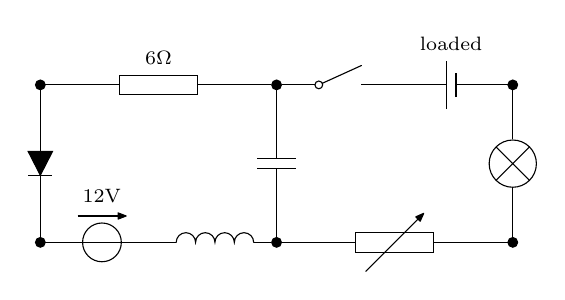
\begin{tikzpicture}[
    circuit ee IEC,
    x = 3cm, y = 2cm,
    every info/.style = {font = \scriptsize},
    set diode graphic = var diode IEC graphic,
    set make contact graphic = var make contact IEC graphic,
  ]
  \foreach \i in {1,...,3} {
    \node [contact] (lower contact \i) at (\i,0) {};
    \node [contact] (upper contact \i) at (\i,1) {};
  }
  \draw (upper contact 1) to [diode] (lower contact 1);
  \draw (lower contact 2) to [capacitor] (upper contact 2);
  \draw (upper contact 1) to [resistor = {ohm = 6}]
        (upper contact 2);
  \draw (lower contact 2) to [resistor = {adjustable}]
        (lower contact 3);
  \draw (lower contact 1) to [
           voltage source = {near start,
                             direction info = {volt = 12}},
           inductor = {near end}]
        (lower contact 2);
  \draw (upper contact 2) to [make contact = {near start},
                              battery = {near end,
                                         info = {loaded}}]
        (upper contact 3);
  \draw (lower contact 3) to [bulb = {minimum height = 0.6cm}]
        (upper contact 3);
\end{tikzpicture}
\end{document}